\documentclass{report}
\usepackage{geometry}
\usepackage{caption}
\usepackage{subcaption} 
\geometry{hmargin = 2cm,vmargin = 2cm}
\usepackage[utf8]{inputenc}
\usepackage[T1]{fontenc}
\usepackage[table]{xcolor}
\usepackage{amssymb}
\usepackage{amsmath}
\usepackage{amsthm}
\usepackage{mathrsfs}
\usepackage{graphicx}
\usepackage{listings}
\usepackage{tikz}
\usepackage{url}
\usetikzlibrary{arrows,positioning, calc}
\tikzstyle{vertex}=[draw,fill=white!15,circle,minimum size=20pt,inner sep=0pt]
\usepackage{color}
\definecolor{darkWhite}{rgb}{0.94,0.94,0.94}
\lstset{
  aboveskip=3mm,
  belowskip=-2mm,
  backgroundcolor=\color{darkWhite},
  basicstyle=\footnotesize,
  breakatwhitespace=false,
  breaklines=true,
  captionpos=b,
  commentstyle=\color{red},
  deletekeywords={...},
  escapeinside={\%*}{*)},
  extendedchars=true,
  framexleftmargin=16pt,
  framextopmargin=3pt,
  framexbottommargin=6pt,
  frame=tb,
  keepspaces=true,
  keywordstyle=\color{blue},
  language=python,
  literate=
  {²}{{\textsuperscript{2}}}1
  {⁴}{{\textsuperscript{4}}}1
  {⁶}{{\textsuperscript{6}}}1
  {⁸}{{\textsuperscript{8}}}1
  {€}{{\euro{}}}1
  {é}{{\'e}}1
  {è}{{\`{e}}}1
  {ê}{{\^{e}}}1
  {ë}{{\¨{e}}}1
  {É}{{\'{E}}}1
  {Ê}{{\^{E}}}1
  {û}{{\^{u}}}1
  {ù}{{\`{u}}}1
  {â}{{\^{a}}}1
  {à}{{\`{a}}}1
  {á}{{\'{a}}}1
  {ã}{{\~{a}}}1
  {Á}{{\'{A}}}1
  {Â}{{\^{A}}}1
  {Ã}{{\~{A}}}1
  {ç}{{\c{c}}}1
  {Ç}{{\c{C}}}1
  {õ}{{\~{o}}}1
  {ó}{{\'{o}}}1
  {ô}{{\^{o}}}1
  {Õ}{{\~{O}}}1
  {Ó}{{\'{O}}}1
  {Ô}{{\^{O}}}1
  {î}{{\^{i}}}1
  {Î}{{\^{I}}}1
  {í}{{\'{i}}}1
  {Í}{{\~{Í}}}1,
  morekeywords={*,...},
  numbers=left,
  numbersep=10pt,
  numberstyle=\tiny\color{black},
  rulecolor=\color{black},
  showspaces=false,
  showstringspaces=false,
  showtabs=false,
  stepnumber=1,
  stringstyle=\color{gray},
  tabsize=4,
  title=\lstname,
}
%pour la compilation minted : C:\Users\Serge\Anaconda3\pkgs\pygments-2.2.0-py37_0\Scripts à ajouter en PATH et 
%remplacer pdflatex -synctex=1 -interaction=nonstopmode %.tex
%par pdflatex -synctex=1 -interaction=nonstopmode --shell-escape %.tex
\title{Quadtree}
\author{Thiziri Baiche \and Charlotte Briquet \and Serge Durand \and Kevin Meetooa}
\graphicspath{ {./images/} }
\begin{document}
\maketitle
\tableofcontents
\section{Introduction}
Les arbres sont une structure de donnée classique, aux nombreuses variations et applications. Notre objectif pour ce projet est d'étudier et d'implémenter des quadtree \footnote{nous utiliserons le terme quadtree dans le reste du rapport, préféré au terme "arbre quaternaire", pas très joli...}, avec plusieurs applications concrètes. Pour bien comprendre les quadtree nous devons d'abord présenter les arbres binaires. Après avoir introduit les notions et le vocabulaire de base sur les arbres binaires nous étudierons en particulier les arbres binaires de recherche avec une première implémentation. En effet les quadtree peuvent être vu comme une extension des arbres binaires de recherche. Nous présentons également des mesures expérimentales de la complexité des méthodes implémentées.
\section{Notations de Landau}
Pour la description des algorithmes et l'analyse de leur complexité on utilisera les notations usuelles (de Landau). On les rappelle ici :
$f$ et $g$ désignent des fonctions de $\mathbb{N}$ dans $\mathbb{N}$.
\begin{itemize}
\item $f \in \mathcal{O}(g)$ si $\exists D > 0$ et $n_0 \geq 0$ tels que $\forall n \geq n_0, f(n) \leq Dg(n)$
\item $f \in \Omega(g)$ si $\exists C >0$ et $n_0 \geq 0$ tels que $\forall n \geq n_0, Cg(n) \leq f(n)$.
\item $f \in \Theta(g)$ si $\exists C>0, D>0$ et $n_0 \geq 0$ tels que $\forall n \geq n_0, Cg(n) \leq f(n) \leq Dg(n)$.
\end{itemize}

Autrement dit : $f \in \mathcal{O}(g)$ si f est inférieure à g à partir d'un certain rang, à une constante multiplicative près. 
De plus on remarque que $f \in \mathcal{O}(g) \iff g \in \Omega(f)$ et $f \in \Theta(g) \iff (f \in \mathcal{O}(g)$ et $f \in \Omega(g))$.
\section{Les Arbres Binaires}
\subsection{Description et vocabulaire des arbres binaires}
\subsubsection{Définitions générales sur les arbres}

Un \textit{arbre} est une structure de donnée hiérarchique définie par un nombre fini de nœuds. Chaque \textit{nœud} est composé d'une \textit{clef}( appelée également \textit{étiquette}) qui représente sa valeur ou l'information associée, et d'un ensemble de références vers d'autres noeuds. On dit que chaque nœud est relié par une \textit{branche}. 
On nomme des nœuds \textit{parents}, \textit{enfants} ou \textit{fils}, \textit{frères}, \textit{ancêtres} ou \textit{descendants}, les nœuds d'un arbre de manière analogue à un arbre généalogique. Dans un arbre, binaire ou non, un noeud a exactement un parent, sauf la \textit{racine} qui n'en a aucun : c'est la particularité de cette structure et ce qui donne le nom d'arbre. 
On dit qu'un noeud qui n'a aucun fils est une \textit{feuille}.
Le \textit{degré} d'un nœud est défini par le nombre de fils qu'il possède. Le degré maximal correspond au degré de l'arbre.
Un arbre \textbf{binaire} est donc un arbre de degré deux, c'est à dire que chaque noeud a au plus deux fils.
La \textit{taille} d'un arbre est son nombre total de nœuds.
Le \textit{chemin} d'un nœud est une suite de nœuds qu'il faut emprunter pour parcourir l'arbre de la racine au nœud en question. On appelle la \textit{longueur} d'un chemin, le nombre de nœuds empruntés.
La \textit{hauteur} (ou profondeur) d'un arbre est la longueur du chemin le plus long.
On considère la racine de l'arbre comme de niveau 1 puis à chaque génération le niveau augmente de 1.
On définit un \textit{sous-arbre} comme un autre arbre formé par un sous-ensemble de nœuds et de branches d'un arbre principal. En effet on peut considérer le fils d'un noeud comme la racine d'un nouvel arbre, un sous-arbre donc. 

Voilà quelques exemples d'arbres :

\subsubsection{Les arbres ordonnés}

On dit qu'un arbre est \textit{ordonné} si tous ses nœuds ont une étiquette supérieure ou égale à celle de chacun de ses enfants s'ils existent. Ainsi, l'étiquette de la racine a la valeur maximale. Pour tout chemin de l'arbre, les étiquettes se succèdent dans un ordre décroissant.

On appelle \textit{tas} ou \textit{arbre tassé} un arbre binaire ordonné presque complet : tous les niveaux de l'arbre binaire sont remplis, sauf peut-être le dernier qui doit est sur la gauche. On parle aussi d'arbre parfait. La structure de tas est notamment utilisée pour le tri par tas. 

\subsubsection{Les arbres d'expression arithmétiques}

Un \textit{arbre binaire d'expression} est un genre d'arbre binaire utilisé pour représenter, comme son nom l'indique, des expressions. Il existe deux types d'expression qu'un arbre binaire peut représenter : algébrique et booléenne.
Les feuilles d'un arbre binaire d'expression sont des quantités (constantes ou variables) numérique dans le cas algébrique et "vrai" ($T$) ou "faux" ($F$) dans le cas booléen.
Les nœuds internes sont des opérateurs : addition ($+$), soustraction ($-$), multiplication ($\times$), division($\div$) et puissance ($\ldots^{\ldots}$) dans le cas algébrique ou des quantificateurs : "et" ($\wedge$), "ou" ($\vee$) et la négation ($\neg$) dans le cas booléen.
Un arbre d'expression est alors évalué en appliquant l'opérateur de la racine au valeurs obtenues en évaluant récursivement les sous-arbres de gauche et de droite, via un parcours postfixe. 
\begin{figure}
\begin{center}
\begin{tikzpicture}[xscale=1,yscale=1]
\tikzstyle{fleche}=[->,>=latex,thick]
\tikzstyle{noeud}=[fill=white,circle]
\tikzstyle{feuille}=[fill=white,circle]
\def\DistanceInterNiveaux{1}
\def\DistanceInterFeuilles{1}
\def\NiveauA{(-0)*\DistanceInterNiveaux}
\def\NiveauB{(-1)*\DistanceInterNiveaux}
\def\NiveauC{(-2)*\DistanceInterNiveaux}
\def\NiveauD{(-3)*\DistanceInterNiveaux}
\def\InterFeuilles{(1)*\DistanceInterFeuilles}
\node[noeud] (R) at ({(2.5)*\InterFeuilles},{\NiveauA}) {$\times$};
\node[noeud] (Ra) at ({(1.5)*\InterFeuilles},{\NiveauB}) {$\div$};
\node[noeud] (Raa) at ({(0.5)*\InterFeuilles},{\NiveauC}) {$-$};
\node[feuille] (Raaa) at ({(0)*\InterFeuilles},{\NiveauD}) {};
\node[feuille] (Raab) at ({(1)*\InterFeuilles},{\NiveauD}) {$8$};
\node[noeud] (Rab) at ({(2.5)*\InterFeuilles},{\NiveauC}) {$+$};
\node[feuille] (Raba) at ({(2)*\InterFeuilles},{\NiveauD}) {$x$};
\node[feuille] (Rabb) at ({(3)*\InterFeuilles},{\NiveauD}) {$5$};
\node[noeud] (Rb) at ({(4.5)*\InterFeuilles},{\NiveauB}) {$\ldots^{\ldots}$};
\node[feuille] (Rba) at ({(4)*\InterFeuilles},{\NiveauC}) {$4$};
\node[feuille] (Rbb) at ({(5)*\InterFeuilles},{\NiveauC}) {$2$};
\draw[fleche] (R)--(Ra);
\draw[fleche] (Ra)--(Raa);
\draw[fleche] (Raa)--(Raab);
\draw[fleche] (Ra)--(Rab);
\draw[fleche] (Rab)--(Raba);
\draw[fleche] (Rab)--(Rabb);
\draw[fleche] (R)--(Rb);
\draw[fleche] (Rb)--(Rba);
\draw[fleche] (Rb)--(Rbb);
\end{tikzpicture}
\caption{Exemple d'arbre binaire d'expression algébrique} \label{fig:Exemple d'arbre binaire d'expression algébrique}
\end{center}
\end{figure} 

\begin{figure}
\begin{center}
\begin{tikzpicture}[xscale=1,yscale=1]
\tikzstyle{fleche}=[->,>=latex,thick]
\tikzstyle{noeud}=[fill=white,circle]
\tikzstyle{feuille}=[fill=white,circle]
\def\DistanceInterNiveaux{1}
\def\DistanceInterFeuilles{1}
\def\NiveauA{(-0)*\DistanceInterNiveaux}
\def\NiveauB{(-1)*\DistanceInterNiveaux}
\def\NiveauC{(-2)*\DistanceInterNiveaux}
\def\NiveauD{(-3)*\DistanceInterNiveaux}
\def\InterFeuilles{(1)*\DistanceInterFeuilles}
\node[noeud] (R) at ({(2.5)*\InterFeuilles},{\NiveauA}) {$\vee$};
\node[noeud] (Ra) at ({(1.5)*\InterFeuilles},{\NiveauB}) {$\wedge$};
\node[noeud] (Raa) at ({(0.5)*\InterFeuilles},{\NiveauC}) {$\neg$};
\node[feuille] (Raaa) at ({(0)*\InterFeuilles},{\NiveauD}) {$F$};
\node[feuille] (Raab) at ({(1)*\InterFeuilles},{\NiveauD}) {};
\node[noeud] (Rab) at ({(2.5)*\InterFeuilles},{\NiveauC}) {$\vee$};
\node[feuille] (Raba) at ({(2)*\InterFeuilles},{\NiveauD}) {$T$};
\node[feuille] (Rabb) at ({(3)*\InterFeuilles},{\NiveauD}) {$F$};
\node[noeud] (Rb) at ({(4.5)*\InterFeuilles},{\NiveauB}) {$\vee$};
\node[feuille] (Rba) at ({(4)*\InterFeuilles},{\NiveauC}) {$T$};
\node[feuille] (Rbb) at ({(5)*\InterFeuilles},{\NiveauC}) {$F$};
\draw[fleche] (R)--(Ra);
\draw[fleche] (Ra)--(Raa);
\draw[fleche] (Raa)--(Raaa);
\draw[fleche] (Ra)--(Rab);
\draw[fleche] (Rab)--(Raba);
\draw[fleche] (Rab)--(Rabb);
\draw[fleche] (R)--(Rb);
\draw[fleche] (Rb)--(Rba);
\draw[fleche] (Rb)--(Rbb);
\end{tikzpicture}
\caption{Exemple d'arbre binaire d'expression booléen} \label{fig:Exemple d'arbre binaire d'expression booléen}
\end{center} 
\end{figure}


\subsection{Particularité des arbres binaires}

On donne la définition inductive de l'ensemble des arbres binaires étiqueté sur un ensemble E, qu'on note AB:
\begin{flushleft}
    \bf
    \underline{Base :}
    
\end{flushleft}
$\emptyset \in AB$ et $\forall x \in E, (x,\emptyset,\emptyset) \in AB$
\begin{flushleft}
    \bf
    \underline{Induction :}
\end{flushleft}
    $\forall x \in E, G \in AB, D \in AB : (x,G,D) \in AB$
    
Un arbre binaire est ainsi un triplet constitué de :
\begin{itemize}
\item un nœud racine
\item un sous-arbre gauche
\item un sous-arbre droit
\end{itemize}
éventuellement vides.

Un arbre binaire qui ne contient pas de nœuds est appelé un arbre vide ou un arbre nul.
Si le sous-arbre de gauche n'est pas vide, sa racine est appelée le fils gauche de la racine de l'arbre entier. Il en va de même pour le sous-arbre de droite.
Par exemple, dans l'arbre (a), le nœud « 2 » est le fils de gauche de la racine de l'arbre, il est aussi la racine du sous-arbre de gauche.
Si un sous-arbre est un arbre nul, on dit alors que le fils est absent ou manquant.
\begin{figure}
\begin{center}
\begin{tikzpicture}[xscale=1,yscale=1]
\tikzstyle{fleche}=[->,>=latex,thick]
\tikzstyle{noeud}=[fill=white,circle]
\tikzstyle{feuille}=[fill=white,circle]
\def\DistanceInterNiveaux{1}
\def\DistanceInterFeuilles{1}
\def\NiveauA{(-0)*\DistanceInterNiveaux}
\def\NiveauB{(-1)*\DistanceInterNiveaux}
\def\NiveauC{(-2)*\DistanceInterNiveaux}
\def\NiveauD{(-3)*\DistanceInterNiveaux}
\def\InterFeuilles{(1)*\DistanceInterFeuilles}
\node[noeud] (R) at ({(2)*\InterFeuilles},{\NiveauA}) {$3$};
\node[noeud] (Ra) at ({(1)*\InterFeuilles},{\NiveauB}) {$2$};
\node[noeud] (Raa) at ({(0.5)*\InterFeuilles},{\NiveauC}) {$1$};
\node[feuille] (Raaa) at ({(0)*\InterFeuilles},{\NiveauD}) {$6$};
\node[feuille] (Raab) at ({(1)*\InterFeuilles},{\NiveauD}) {};
\node[feuille] (Rab) at ({(2)*\InterFeuilles},{\NiveauC}) {$4$};
\node[noeud] (Rb) at ({(3.5)*\InterFeuilles},{\NiveauB}) {$7$};
\node[feuille] (Rba) at ({(3)*\InterFeuilles},{\NiveauC}) {$5$};
\node[feuille] (Rbb) at ({(4)*\InterFeuilles},{\NiveauC}) {};
\draw[fleche] (R)--(Ra);
\draw[fleche] (Ra)--(Raa);
\draw[fleche] (Raa)--(Raaa);
\draw[fleche] (Ra)--(Rab);
\draw[fleche] (R)--(Rb);
\draw[fleche] (Rb)--(Rba);
\end{tikzpicture}
\end{center}
\caption{Arbre (a)} \label{fig:Exemples d'arbres}
\end{figure}

\begin{figure}
\begin{center}
\begin{tikzpicture}[xscale=1,yscale=1]
\tikzstyle{fleche}=[->,>=latex,thick]
\tikzstyle{noeud}=[fill=white,circle]
\tikzstyle{feuille}=[fill=white,circle]
\def\DistanceInterNiveaux{1}
\def\DistanceInterFeuilles{1}
\def\NiveauA{(-0)*\DistanceInterNiveaux}
\def\NiveauB{(-1)*\DistanceInterNiveaux}
\def\NiveauC{(-2)*\DistanceInterNiveaux}
\def\NiveauD{(-3)*\DistanceInterNiveaux}
\def\InterFeuilles{(1)*\DistanceInterFeuilles}
\node[noeud] (R) at ({(2)*\InterFeuilles},{\NiveauA}) {$3$};
\node[noeud] (Ra) at ({(1)*\InterFeuilles},{\NiveauB}) {$2$};
\node[noeud] (Raa) at ({(0.5)*\InterFeuilles},{\NiveauC}) {$1$};
\node[feuille] (Raaa) at ({(0)*\InterFeuilles},{\NiveauD}) {};
\node[feuille] (Raab) at ({(1)*\InterFeuilles},{\NiveauD}) {$6$};
\node[feuille] (Rab) at ({(2)*\InterFeuilles},{\NiveauC}) {$4$};
\node[noeud] (Rb) at ({(3.5)*\InterFeuilles},{\NiveauB}) {$7$};
\node[feuille] (Rba) at ({(3)*\InterFeuilles},{\NiveauC}) {};
\node[feuille] (Rbb) at ({(4)*\InterFeuilles},{\NiveauC}) {$5$};
\draw[fleche] (R)--(Ra);
\draw[fleche] (Ra)--(Raa);
\draw[fleche] (Raa)--(Raab);
\draw[fleche] (Ra)--(Rab);
\draw[fleche] (R)--(Rb);
\draw[fleche] (Rb)--(Rbb);
\end{tikzpicture}
\end{center}
\caption{Arbre (b)} \label{fig:Exemples d'arbres}
\end{figure}

\begin{figure}
\begin{center}
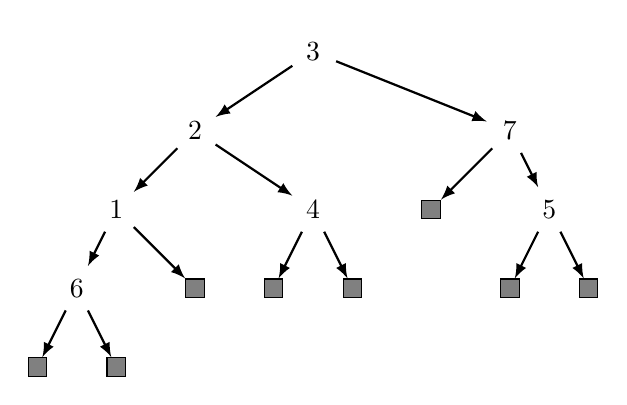
\begin{tikzpicture}[xscale=1,yscale=1]
\tikzstyle{fleche}=[->,>=latex,thick]
\tikzstyle{noeud}=[fill=white,circle]
\tikzstyle{feuille}=[fill=gray,draw]
\def\DistanceInterNiveaux{1}
\def\DistanceInterFeuilles{1}
\def\NiveauA{(-0)*\DistanceInterNiveaux}
\def\NiveauB{(-1)*\DistanceInterNiveaux}
\def\NiveauC{(-2)*\DistanceInterNiveaux}
\def\NiveauD{(-3)*\DistanceInterNiveaux}
\def\NiveauE{(-4)*\DistanceInterNiveaux}
\def\InterFeuilles{(1)*\DistanceInterFeuilles}
\node[noeud] (R) at ({(3.5)*\InterFeuilles},{\NiveauA}) {$3$};
\node[noeud] (Ra) at ({(2)*\InterFeuilles},{\NiveauB}) {$2$};
\node[noeud] (Raa) at ({(1)*\InterFeuilles},{\NiveauC}) {$1$};
\node[noeud] (Raaa) at ({(0.5)*\InterFeuilles},{\NiveauD}) {$6$};
\node[feuille] (Raaaa) at ({(0)*\InterFeuilles},{\NiveauE}) {};
\node[feuille] (Raaab) at ({(1)*\InterFeuilles},{\NiveauE}) {};
\node[feuille] (Raab) at ({(2)*\InterFeuilles},{\NiveauD}) {};
\node[noeud] (Rab) at ({(3.5)*\InterFeuilles},{\NiveauC}) {$4$};
\node[feuille] (Raba) at ({(3)*\InterFeuilles},{\NiveauD}) {};
\node[feuille] (Rabb) at ({(4)*\InterFeuilles},{\NiveauD}) {};
\node[noeud] (Rb) at ({(6)*\InterFeuilles},{\NiveauB}) {$7$};
\node[feuille] (Rba) at ({(5)*\InterFeuilles},{\NiveauC}) {};
\node[noeud] (Rbb) at ({(6.5)*\InterFeuilles},{\NiveauC}) {$5$};
\node[feuille] (Rbba) at ({(6)*\InterFeuilles},{\NiveauD}) {};
\node[feuille] (Rbbb) at ({(7)*\InterFeuilles},{\NiveauD}) {};
\draw[fleche] (R)--(Ra);
\draw[fleche] (Ra)--(Raa);
\draw[fleche] (Raa)--(Raaa);
\draw[fleche] (Raaa)--(Raaaa);
\draw[fleche] (Raaa)--(Raaab);
\draw[fleche] (Raa)--(Raab);
\draw[fleche] (Ra)--(Rab);
\draw[fleche] (Rab)--(Raba);
\draw[fleche] (Rab)--(Rabb);
\draw[fleche] (R)--(Rb);
\draw[fleche] (Rb)--(Rba);
\draw[fleche] (Rb)--(Rbb);
\draw[fleche] (Rbb)--(Rbba);
\draw[fleche] (Rbb)--(Rbbb);
\end{tikzpicture}
\end{center}
\caption{Arbre (c)} \label{fig:Exemples d'arbres}
\end{figure}

Un arbre binaire de recherche n'est pas seulement un arbre ordonné où chaque nœud a un degré maximal de 2.  En effet, pour une racine n'ayant qu'un seul fils, sa position, s'il s'agit du fils de gauche ou du fils de droite, importe contrairement à un arbre ordonné.
La figure 1 représente des arbres binaires dessinés sous leur forme standard. Attention, l'arbre (a) est différent de l'arbre (b) quand ils sont considérés comme des arbres binaires, mais en tant que arbres classiques, ils sont identiques.
Cependant, un arbre binaire peut être associé à un arbre ordonné en ajoutant une représentation explicite des informations manquantes comme dans l'arbre (c). L'idée est de remplacer chaque enfant manquant de l'arbre binaire par un nœud n'ayant aucune descendance. Ces nœuds sont appelés des feuilles et sont représentés par des carrés dans l'arbre (c). On parle aussi de nœud externe pour une feuille en opposition aux nœuds internes. On obtient alors un arbre binaire entier : chaque nœud est soit une feuille soit a un degré égal à 2. Il n'y a pas de nœud de degré 1.





\section{Les arbres binaires de recherche}
\subsection{Définition}
Un arbre binaire de recherche est un arbre binaire étiqueté sur un ensemble muni d'un ordre total (typiquement les réels ou les entiers) dans lequel tout noeud a une étiquette supérieure à celles de tout les noeuds de son sous arbre gauche et inférieure à celles de son sous arbre droit. L'abbréviation ABR ou BST pour \textit{binary search tree} est fréquemment utilisée. On donne aussi la définition inductive suivante :
\begin{flushleft}
    \bf
    \underline{Base :}
    
\end{flushleft}
$\emptyset \in ABR$, $\forall x \in E, (x,\emptyset, \emptyset) \in ABR$
\begin{flushleft}
    \bf
    \underline{Induction :}
\end{flushleft}
    $\forall x \in E, G \in ABR, D \in ABR$, si :
    \begin{itemize}
        \item $\forall (x_1,G_1,D_1) \in G, x_1 < x$
        \item $\forall (x_2,G_2,D_2) \in D, x_2 > x$
    \end{itemize}
    alors $(x,G,D) \in ABR$

\subsection{Propriétés remarquables sur les arbres binaires de recherche}

%Je vais ajouter les résultats et preuves sur la tailles d'un ABR parfait, la hauteur moyenne d'un noeud, etc...%
\subsection{Parcours et affichage}

Pour réaliser les différents parcours décrits ci-dessous, on peut définir un arbre par un dictionnaire qui associe chaque nœud à ses fils. Par exemple, l'arbre (a) est définit par :
\begin{lstlisting}
A = {3:[2, 7], 2:[1, 4], 7:[5], 1:[6], 4:[], 5:[], 6:[]}
\end{lstlisting}
C'est cette méthode qui est utilisée pour décrire un arbre dans le cas du parcours en largeur. Cependant, on peut également définir une classe Arbre telle que :
\begin{lstlisting}
class Arbre: 
    def __init__(self,valeur): 
        self.gauche = None
        self.droit = None
        self.racine = valeur
# L'arbre (a) est donc défini par :
A = Arbre(3) 
A.gauche = Arbre(2) 
A.droit = Arbre(7) 
A.gauche.gauche = Arbre(1) 
A.gauche.droit = Arbre(4)
A.gauche.gauche.gauche = Arbre(6)
A.droit.gauche = Arbre(5)
\end{lstlisting}
On utilisera cette classe pour les parcours en profondeur.
\subsubsection{Parcours en largeur}
Le principe d'un parcours en largeur est de lister les nœuds de l'arbre niveau par niveau en commençant par les nœuds de niveau 1 puis les nœuds de niveau 2 et ainsi de suite. Dans chaque niveau, les nœuds sont parcourus de gauche à droite.
Le parcours en largeur de l'arbre (a) est donc $[3, 2, 7, 1, 4, 5, 6]$.
Contrairement aux parcours suivant le parcours en largeur s'implémente naturellement par un algorithme itératif.
L'algorithme d'un tel parcours se fait à l'aide d'une file (premier entré, premier sorti). On enfile d'abord la racine puis on utilise une boucle tant que la file n'est pas vide.
On défile la racine que l'on traite (typiquement par un affichage mais cela peut être un autre traitement), on enfile les fils de la racine en commençant par le fils gauche et on répète la boucle. Et ainsi de suite jusqu'à ce que la file soit vide.
\begin{lstlisting}
def parcours_largeur(arbre, racine):
	liste = [racine]
	parcours = [racine]
	while liste :
		x = liste.pop(0)
		for fils in arbre[x]:
			if fils in liste : 
				continue
			parcours.append(fils)
			liste.append(fils)
	return parcours
\end{lstlisting}
Pour les arbres la complexité d'un tel parcours est en $\Theta(n)$ : on fait exactement n tour de boucle. 
Remarquons que cet algorithme peut être utilisé sur n'importe quel type d'arbre, et même sur des graphes en général, avec quelques modifications pour ne pas repasser sur le même noeud et avoir une boucle infinie dans le cas de graphe cyclique par exemple.

\subsubsection{Parcours en profondeur}
Le principe d'un parcours en profondeur est de lister les nœuds de l'arbre récursivement à partir de la racine puis les sous-arbres gauches et droits de cette racine et ainsi de suite pour la totalité de l'arbre.
Il existe plusieurs types de parcours en profondeur : Infixe, Suffixe (ou Postfixe) et Préfixe.
\begin{itemize}
\item Infixe

Le parcours infixe consiste à lister les nœuds en partant du sous-arbre gauche puis remonter à sa racine et enfin parcourir le sous-arbre droit.
Le parcours infixe de l'arbre (a) est donc $[6, 1, 2, 4, 3, 5, 7]$.
\begin{lstlisting}
def parcours_infixe(arbre): 
    if arbre: 
        parcours_infixe(arbre.gauche) 
        print(arbre.racine)
        parcours_infixe(arbre.droit) 
\end{lstlisting}

\item Suffixe

Le parcours suffixe consiste quant à lui à lister les nœuds depuis le sous-arbre gauche puis le sous-arbre droit et enfin remonter à la racine.
Le parcours suffixe de l'arbre (a) est donc $[6, 1, 4, 2, 5, 7, 3]$.
\begin{lstlisting}
def parcours_suffixe(arbre): 
     if arbre: 
        parcours_suffixe(arbre.gauche) 
        parcours_suffixe(arbre.droit) 
        print(arbre.racine)
\end{lstlisting}

\item Préfixe

Le parcours préfixe, finalement, consiste à lister les nœuds en commençant par la racine puis le sous-arbre gauche et enfin le sous-arbre droit.
Le parcours préfixe de l'arbre (a) est donc $[3, 2, 1, 6, 4, 7, 5]$.
\begin{lstlisting}
def parcours_prefixe(arbre):
    if arbre:
        print(arbre.racine)
        parcours_prefixe(arbre.gauche)
        parcours_prefixe(arbre.droit)
\end{lstlisting}

\end{itemize}

Dans les trois cas la complexité est également en $\Theta(n)$, on passe exactement une fois sur chaque noeud. 
\subsection{méthodes principales}
\subsubsection{recherche :} 
La recherche se fait aussi de manière récursive l'algorithme est assez simple :
\\soit x l'élément qu'on cherche
\\- on regarde si x est égale à la racine dans ce cas on renvoi directement la racine 
\\- si x est plus petit que la racine (x est donc forcement dans le sous arbre gauche) on fait un appel récursif sur le sous arbre gauche 
\\- si x est plus grand que la racine on fait un appel récursif sur le sous arbre droit 
\\- et si on atteint une feuille et que sa clé n'est pas l'élément qu'on recherche ça veut dire que l'élément ne se trouve pas dans l'arbre.
\subsubsection{insertion}
Pour l'insertion on procède de manière analogue à la recherche : pour insérer un élément il faut savoir dans quelle partie de l'arbre le mettre pour que cela reste un arbre binaire de recherche.
Pour cela il suffit de comparer la valeur à insérer au noeud courant. On distingue trois cas :
\begin{enumerate}
    \item les valeurs sont égales : on fait un retour, il n'y a rien à insérer. On rappelle que dans un arbre binaire de recherche les étiquettes des noeuds sont distinctes.
    \item la valeur à insérer est plus petite que le noeud courant. On a alors deux possibilités :
    \begin{itemize}
        \item le sous arbre gauche est vide : on procède à l'insertion en créant un noeud avec pour étiquette la valeur à insérer, et des sous arbres gauche et droit vides.
        \item le sous arbre gauche n'est pas vide : on fait un appel récursif sur cet arbre.
    \end{itemize}
    \item si elle est plus grande on procède de manière analogue sur le sous arbre droit.
\end{enumerate}
On remarque que dans cette version on insère toujours au niveau des feuilles, si insertion il y a. L'algorithme est simple, mais il n'est pas optimal sur la structure de l'arbre, dans le sens où on ne cherche pas à garantir une structure équilibrée. Nous verrons plus tard (c'est prévu pour le rapport final) qu'il est possible de le faire en introduisant la rotation d'arbre.
La complexité est en $\mathcal{O}(h)$ avec $h$ la hauteur de l'arbre, comme pour la recherche. La preuve est tout à fait analogue à la preuve de la méthode recherche.
\subsubsection{suppression}
La fonction de suppression se fait de manière récursive. Elle est assez simple mais il faut juste faire attention à ne pas perdre des informations ou à modifier la structure d'arbre :
\\L'algorithme est le suivant:
\\soit x l'élément qu'on veut supprimer :
\\- si x c'est la racine de notre arbre, il y a trois cas à traiter :
\\	- si x n'a pas de fils on le supprime directement
\\	- si x a un seul fils on le remplace par celui-ci
\\  - s'il en a deux on échange le x soit avec le max du sous arbre gauche (qui correspond au fils le plus a droite du sous arbre gauche), soit avec le min du sous arbre droit(qui correspond au fils le plus 
a gauche du sous arbre droit), puis on supprime le max ou le min d'après ce qu'on a choisit en faisant un appel récursif .
\\- si x est plus petit que la racine on fait un appel récursif sur le sous arbre gauche 
\\- si x est plus grand on fait un appel récursif sur le sous arbre droit .

\subsection{Complexité des méthodes principales}
\subsubsection{Protocole expérimental:}
\subsubsection{Pire cas:}
Comme expliqué dans la partie théorique, le pire cas pour les fonctions de recherche est le cas où l'on doit parcourir l'arbre jusqu'à arriver à une feuille.
Nous avons modélisé ce cas par des arbres de hauteur égale à leur nombre de sommet. \\
Graphiquement, cela correspond à des arbres qui ont uniquement des fils gauche ou uniquement des fils droit. Voici un exemple de tel arbre de taille 3:

\begin{center}
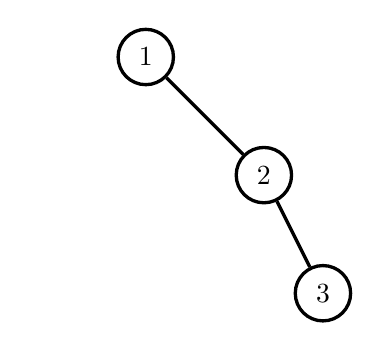
\begin{tikzpicture}[very thick,level/.style={sibling distance=30mm/#1}]
\node [vertex] {$1$}
   child{edge from parent[draw=none]}
   child {
    node [vertex]  {$2$}
    child{edge from parent[draw=none]}
    child{node [vertex] {$3$}}
   };
\end{tikzpicture}
\end{center}

Nous avons utilisé l'implémentation des arbres binaires de recherche en python.
Nous avons crée de tels arbres de taille allant de 1000 à 100 000 noeuds. Il nous était impossible d'aller plus haut sans faire crasher python.\\

Pour chaque arbre, nous appelons la fonction étudiée sur une feuille de l'arbre (dans ce cas, il s'agit simplement du noeud de plus grande étiquette) et mesurons le temps que cela prend à l'aide du module time.timeit. \\
Nous répétons cette opération 100 fois et cela nous permet de faire une moyenne pour chaque arbre. Nous pouvons ensuite tracer le temps d'exécution en fonction du nombre de noeuds.\\
Voici les résultats obtenus: \\
\includegraphics[scale=0.65]{images/rech.jpg} \\
\includegraphics[scale=0.65]{images/ins.jpg} \\
\includegraphics[scale=0.65]{images/supp.jpg}


\subsubsection{Cas moyen:}
Le cas moyen correspond au cas où l'arbre binaire de recherche est de hauteur logarithmique. En effet, un théorème indique que la hauteur d'un arbre généré aléatoirement sera en moyenne logarithmique.

Nous avons modélisé ce cas par des arbres parfaits car d'après la partie théorique, la hauteur d'un arbre parfait est en $\Theta$ (n)

\section{Implémentation : comparaison entre structure récursive et représentation en liste}
\subsection{Structure récursive}
Une représentation qui semble la plus naturelle est d'implémenter une structure avec auto-référence. En effet en s'inspirant de la définition inductive on peut voir un arbre binaire comme une structure contenant essentiellement 3 champs : une clef et deux arbres binaires, ses sous-arbres gauche et droit. 

En terme d'implémentation cela dépend du langage utilisé. 
En C cela passera par la création d'un type spécifique arbre avec en variable des pointeurs vers des variables de ce même type, en plus d'une variable clef de type entier par exemple. 
En suivant le paradigme de la programmation objet (typiquement en java ou en Python), on créé une classe arbre ayant deux attributs de type arbre en plus de l'attribut clef (et d'autres attributs si nécessaires). La souplesse de Python sur les types rend la création de la classe particulièrement aisée mais il faudra être vigilant sur l'utilisation. 

On pourra déclarer la classe comme ceci :

\begin{lstlisting}
class ArbreBinaire():
    def __init__(self,clef,gauche = None ,droite = None):
        """ Anything x ArbreBinaire x ArbreBinaire -> ArbreBinaire
        Constructeur d'arbre"""
        self.clef = clef
        self.gauche = gauche
        self.droite = droite
\end{lstlisting}

Exemple d'instanciation :

\begin{lstlisting}
Feuille1 = ArbreBinaire(1)
Feuille2 = ArbreBinaire(2)
Arbre = ArbreBinaire(3,Feuille1,Feuille2)
\end{lstlisting}

L'arbre créé est :
\begin{center}
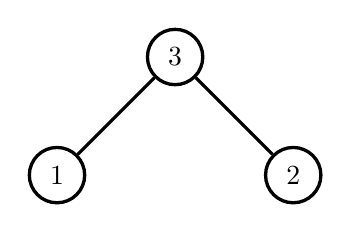
\begin{tikzpicture}[very thick,level/.style={sibling distance=30mm/#1}]
\node [vertex] (r){$3$}
  child {
    node [vertex] (a) {$1$}
   }
   child {
    node [vertex] (a) {$2$}
   }
   
   ;
\end{tikzpicture}
\end{center}

\subsection{Liste}

On peut aussi représenter l'arbre sous forme de liste. L'idée est d'avoir la racine au début de la liste, le fils gauche à l'index 1, le fils droite à l'index 2 et ainsi de suite. Pour un nœud à l'indice i, on trouve son fils gauche à l'indice 2i de la liste, et le droit à l'indice 2i+1. 
On peut donc également retrouver le père d'un nœud facilement : pour un nœud d'index i, le père est à l'index $\lfloor \frac{i-1}{2} \rfloor$ (on prend la partie entière dans la division par 2).
On fera attention à ne pas sauter les nœuds vides, il faut bien les représenter dans la liste par un caractère spécial en fonction de ce que l'arbre contient comme type de donnée. Par exemple mettre False pour un arbre contenant des entiers éventuellement nuls n'est pas une bonne solution, le test False == 0 renvoyant true en Python (et beaucoup d'autres langages).
Par exemple l'arbre suivant :

\begin{center}
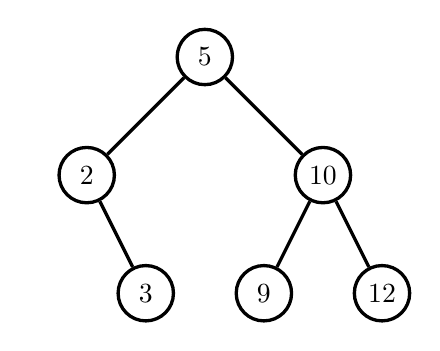
\begin{tikzpicture}[very thick,level/.style={sibling distance=30mm/#1}]
\node [vertex] {$5$}
  child {
    node [vertex]  {$2$}
    child{edge from parent[draw=none]}
    child{node [vertex] {$3$}}
   }
   child {
    node [vertex] {$10$}
    child{node [vertex] {$9$}}	
    child{node [vertex] {$12$}}
   };
\end{tikzpicture}
\end{center}

sera représenté par la liste :
$[5,2,10,"vide",3,9,12]$

Remarquons qu'idéalement il faut utiliser une structure de base qui combine les avantages de la liste chaînée et des tableaux : nous avons besoins d'accéder à aux éléments à une position précise en temps constant si possible, mais la structure doit être de taille flexible pour l'agrandir ou la réduire. 

\subsection{Comparaison}
\subsubsection{Avantages et inconvénients}
Pour la structure récursive :
\begin{itemize}
\item[•]
Lisibilité du code.
\item[•]
Gain mémoire pour les arbres avec des nœuds vides : on n'insère que les nœuds non vide dans l'arbre.
\item[•]
Plus grande souplesse dans le type de donnée représentée dans le nœud.
\end{itemize}
\paragraph*{}
Pour la représentation en liste :
\begin{itemize}
\item[•]
Gain de mémoire pour les arbres pleins ou parfait.
\item[•]
Simplicité de la mise en place, notamment pour les langages implémentant déjà une structure de liste / tableau (en Python on dispose par exemple déjà des primitives append, pop, len etc).
\item[•]
Accès immédiat au parent.
\end{itemize}
Les inconvénients se déduisent des avantages : pour la structure récursive elle est plus lourde à mettre en place, ça peut être lourd en mémoire pour des arbres pleins.
Pour la liste, le code sera peut être moins lisible et surtout on gâche de la mémoire lorsque l'arbre contient des nœuds vide. 

Dans certains cas la liste est particulièrement appropriée par exemple pour la représentation des tas (arbre binaire parfait sur un ensemble totalement ordonnée où les chemins de la racine vers les feuilles sont toujours croissant), utilisés dans le tri par tas où le but est d'ordonner une liste. 

Pour notre implémentation nous avons choisi la représentation en structure récursive en utilisant la programmation orientée objet en Python.

\section{Conclusion}

\nocite{*}
\bibliographystyle{plain}
\bibliography{biblio}

\end{document}
